\section{Durchf\"uhrung}
\label{sec:Durchfuehrung}
Gemessen wird die Anzahl der Zerfälle $n$ für einen bestimmten Zeitraum $\Delta{t}$. Dieser muss angemessen gewählt werden. Ist $\Delta{t}$ zu groß ergibt sich ein systematischer Fehler; ist $\Delta{t}$ zu klein verfälschen statistische Fehler die Messung.
Es werden die Isotope \ce{^115 In} und \ce{^103 Rh} verwendet und für $\Delta{t_\mathup{In}=250\,\si\second}$ und $\Delta{t_\mathup{Rh}=20\,\si\second}$ die Anzahl $n$ gemessen.
Aktiviert werden die Proben indem sie sich vor der Messung in den Aktivierungsschächten befinden, gezeigt in Abbildung \ref{fig:aktivierung}. Für die eigentliche Messung werden die Proben in die Apparatur, gezeigt in Abbildung \ref{fig:apparatur} eingesetzt. Ein Mantelzählrohr liefert für jeden Zerfall einen Impuls am Verstärkerausgang. Dieser wird vom Zählwerk regestriert. Ist der Zeitraum $\Delta{t}$ abgelaufen, wird auf ein zweites Zählwerk umgeschaltet und der Wert $n$ kann notiert werden. Für Indium wird 16 Mal eine Messung für $\Delta{t_\mathup{In}}=250\,\si\second$ druchgeführt; für Rhodium werden $37$ Mal die Zerfälle pro Zeiteinheit $\Delta{t_\mathup{Rh}}=20\,\si\second$ gemessen.
\begin{figure}[p]
	\centering
	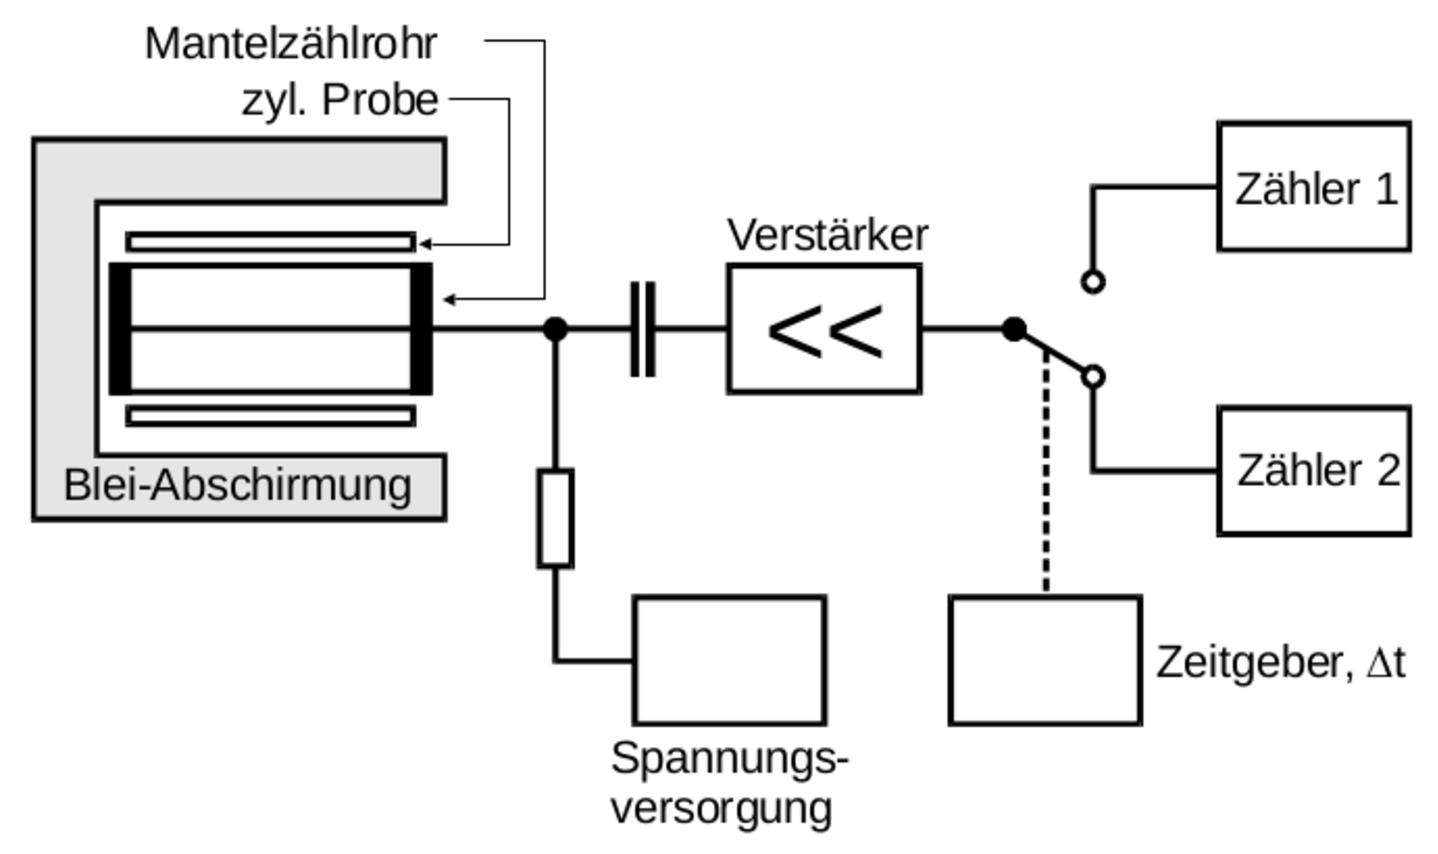
\includegraphics[width=0.7\textwidth]{Bilder/Aktivierung.pdf}
	\caption{Schichtdicke $d$ aufgetragen gegen die Strahlungsintensität.}
	\label{fig:apparatur}
\end{figure}

\begin{figure}[p]
	\centering
	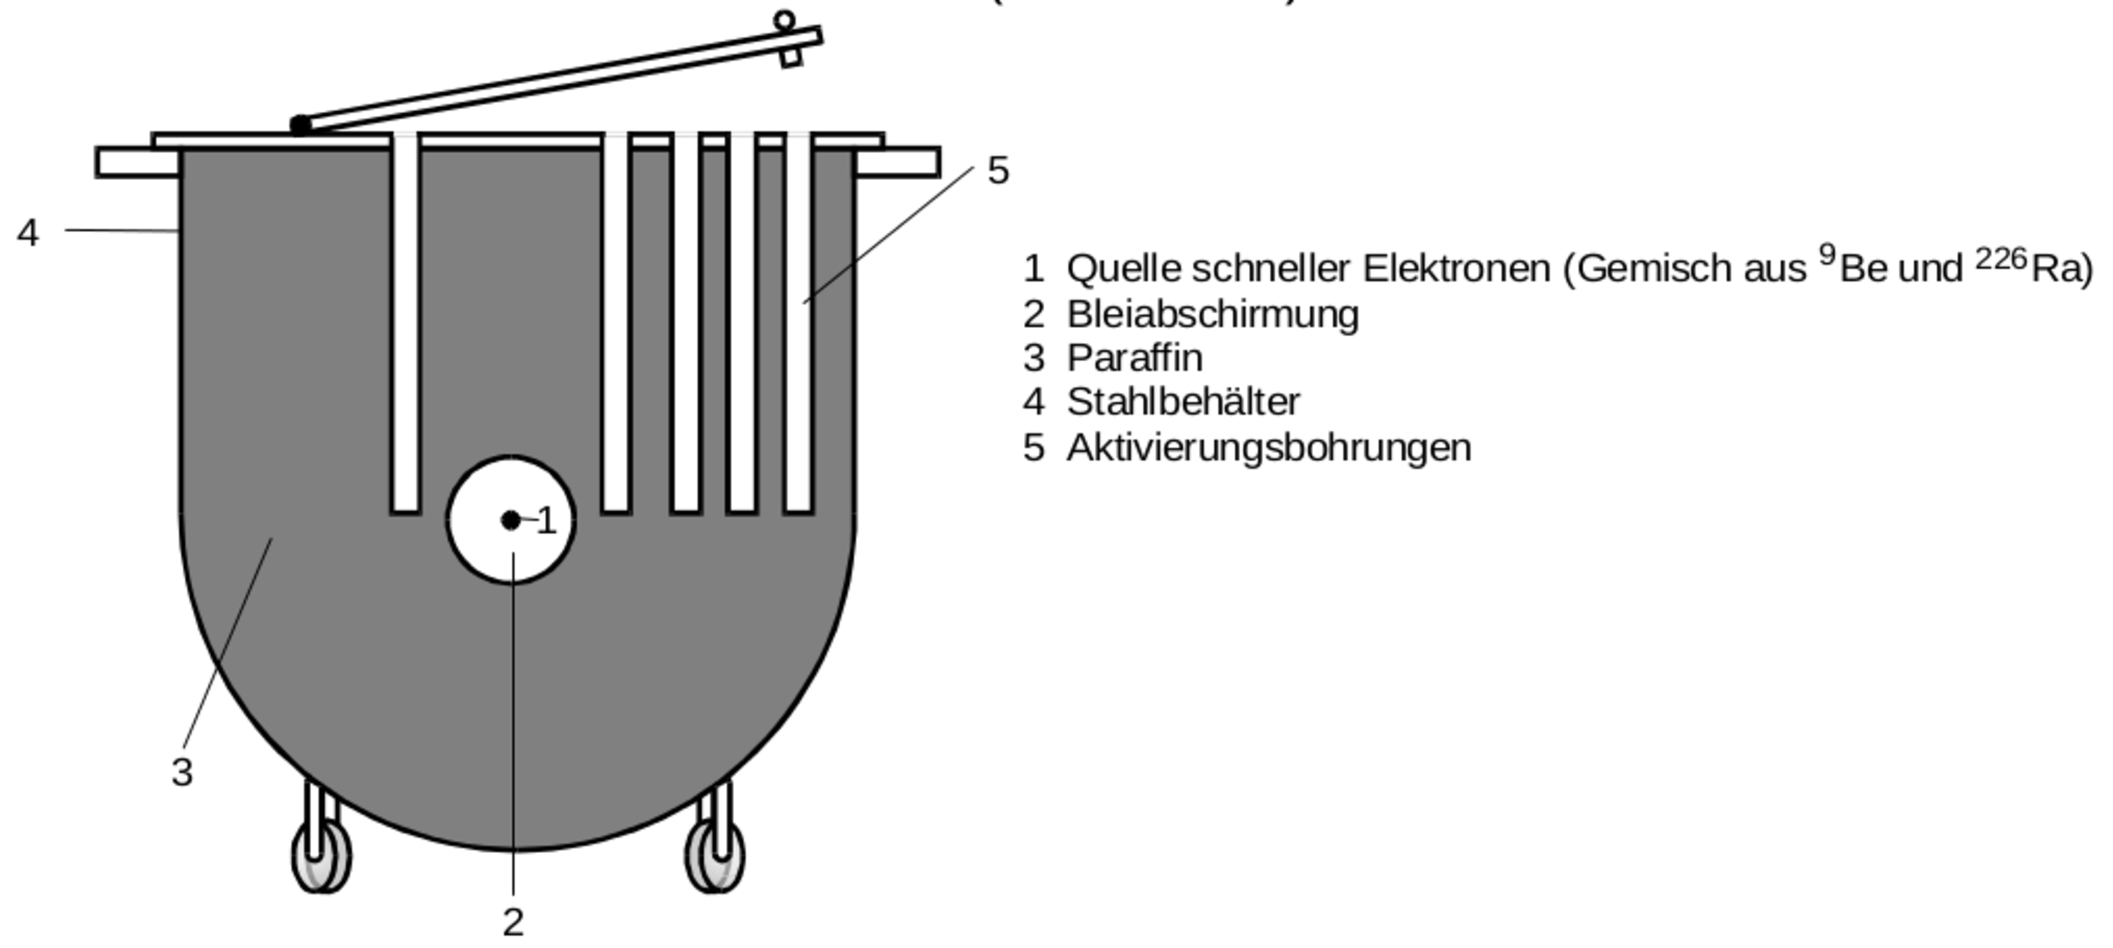
\includegraphics[width=0.8\textwidth]{Bilder/wirklicheAktivierung.pdf}
	\caption{Schichtdicke $d$ aufgetragen gegen die Strahlungsintensität.}
	\label{fig:aktivierung}
\end{figure}
\newpage